\chapter{Configuración red LAN}\label{ch:red lan}

	\section{¿Que es una red LAN?}
	
		Una red LAN es un grupo de dispositivos (impresoras, sistemas, dispositivos móviles, consolas de juegos) interconectados mediante alguna tecnología, y que comparten datos entre sí. Una LAN puede ser una entidad autónoma e independiente, así como una parte de redes más grandes y extensas.\par

		
	\section{¿Que es una dirección IP?}
		
		una dirección IP (Internet Protocol que corresponde al nivel de red del modelo TCP/IP) es un número que identifica, de manera lógica y jerárquica, a una Interfaz red de un dispositivo. En un paquete IP, el
		encabezado contiene una dirección de 32 bits (IPv4) o 128 bits (IPv6). Este identificador es único y no se repite en ningún otro equipo en el mundo y tiene la tarea de registrar el equipo a la red global. Pero una dirección IP no solo la poseen los equipos de cómputo, también los módems, routers, sitios web, etc.\par
		
		Entendiendo el papel de una dirección IP es necesario saber que existen dos tipos de direcciones IP y que se manejan dos protocolos para éstas. Éstos son el protocolo IPv4, pero con la demanda cada día mayor de solicitudes de direcciones IP se está implementando el protocolo IPv6. El cual ofrece mayor direcciones.\par En el mundo del direccionamiento IP se encuentran dos tipos de direcciones IP, estática y dinámica. \par
		
		\subsection{Direcciones IP dinámicas}
			
			Son direcciones variables, entregadas y administradas por un servidor DHCP y su funcionamiento radica en el arrendamiento de esta dirección por un tiempo específico, luego de este periodo de tiempo la dirección se renovará modificando su sintaxis.\par
		
			
		\subsection{Direcciones IP estáticas}\par
			
			Como su nombre lo indica, son direcciones IP que permanecerán fijas, sin ningún tipo de variación. Son usadas en servidores, máquinas de producción conectadas a la red y en general todo usuario que no requiere que su IP sea modificada, ya que de él dependen otros servicios.
	
			
	\section{Configuración de red}	
	
		Por simplicidad y dado que la red del aula es una red pequeña las direcciones IP para los ordenadores de escritorios serán dinámicas. El servidor recibirá una dirección IP estática para que las estaciones de trabajo puedan encontrarlo en la red.\par
	
		La red tendrá la dirección IP 192.168.1.0/24 y se establecerá la dirección IP en 192.168.1.222 para el servidor Docker .\par
		
		\subsection{Diagrama de red}
				
			El diagrama de red es la representación visual de los ordenadores que compondrán la red de trabajo y su interconexión.\par
			
			\begin{figure}[h]
				\centering
				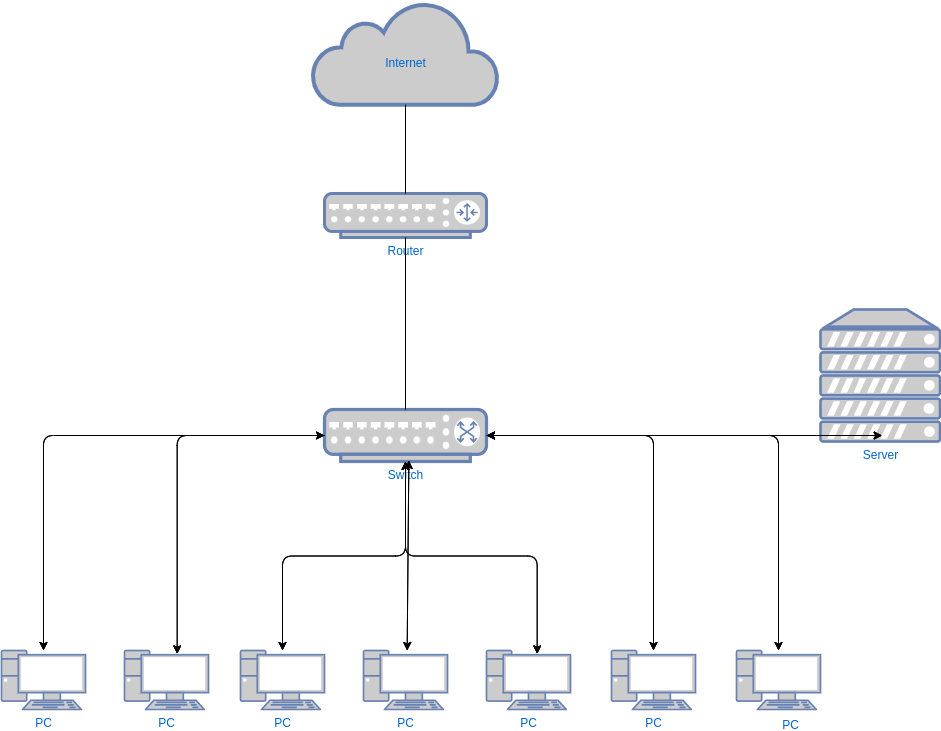
\includegraphics[height=0.6\textwidth]{imagenes/red/diagrama.png}
				\caption{Diagrama de red}
				\label{fig:red local lan}
			\end{figure}
			
				
